\documentclass[12pt,a4paper,oneside]{book} % twoside for draf

%\usepackage{babel}
%\usepackage[utf8]{vietnam}
%\usepackage{times}
%\usepackage{graphicx}

\usepackage[utf8]{inputenc}
\usepackage{mathptmx}	% same Time New Roma
%\renewcommand{\rmdefault}{phv} % Arial
%\renewcommand{\sfdefault}{phv} % Arial

\usepackage{fancyhdr}
\usepackage{algorithm2e}

\usepackage{uitthesis}

%\csdeptname{KHOA ĐIỆN ĐIỆN TỬ}
%\crname{BÁO CÁO THỰC TẬP TỐT NGHIỆP}
% \crname{BÁO CÁO TIỂU LUẬN}
\title{TÊN LUẬN VĂN / ĐỒ ÁN}
\cstuname{SVTH: Donald Trump2}
\csCouncil{Khoa học máy tính}
\csSupervise{PGS. TS. Phạm Hồng Luân}
\csReviewer{TS. Pham Van Hai}
\cttime{1/2016}

\thesislayout

\begin{document}
%-	Bìa cứng - màu xanh dương, chữ mạ vàng (xem mẫu đính kèm)
%-	Trang tên (tờ lót): chất liệu giấy, nội dung giống như bìa LV
%-	Ở gáy LV: in nhan đề LV (có thể in tóm tắt nếu nhan đề quá dài), size 15 – 17
%-	Phiếu Nhiệm vụ LV, chấm điểm Hướng dẫn & Phản biện (đã ký): nhận từ GVHD & GVPB sau khi bảo vệ (theo lịch hẹn).
%-	Lời cam đoan
%-	Lời cảm ơn/ Lời ngỏ
%-	Tóm tắt LV
%-	Mục lục
%-	Danh mục, bảng biểu, hình ảnh, ... (nếu có)
%-	Nội dung LV
%-	Danh mục TL tham khảo
%-	Phụ lục (nếu có)

\coverpage

\frontmatter

% add content here
%-	Lời cam đoan
\begin{declaration}
	Tôi xin cam đoan...
\end{declaration}

%-	Lời cảm ơn/ Lời ngỏ
\begin{acknowledgments}
	Tôi xin chân thành cảm ơn ...
\end{acknowledgments}

%-	Tóm tắt LV
\begin{abstract}
	Tóm tắt luận văn ...
\end{abstract}	
	
\tableofcontents
%\listofsymbols
\listoftables
\listoffigures
%\listofalgorithms


\mainmatter

\fancyhead{}  % Clears all page headers and footers
%\rhead{\thepage}  % Sets the right side header to show the page number
%\lhead{}  % Clears the left side page header
%\fancyfoot[positions]{footer}
\renewcommand{\footrulewidth}{0.4pt}

\pagestyle{fancy}  % Finally, use the "fancy" page style to implement the FancyHdr headers

In this research, we study the problem of stock market forecasting using Recurrent
Neural Network(RNN) with Long Short-Term Memory (LSTM). The purpose of this
research is to examine the feasibility and performance of LSTM in stock market
forecasting. We optimize the LSTM model by testing different configurations, i.e., the
number of neurons in hidden layers and number of samples in sequence. Instead of
using daily stock price data, we collect hourly stock data from the IQFEED database in
order to train our model with relatively low noise samples. Nevertheless, based on the
prediction results of LSTM model, we build up a stock database with six U.S market
stocks from five different industries. The average test accuracy of these six stocks is
54.83%, where the highest accuracy is at 59.5% while the lowest is at 49.75%. We then
develop a trade simulator to evaluate the performance of our model by investing the
portfolio within a period of 400 hours, the total profit gained by the model is
$413,233.33 with $6,000,000 initial investment.
% !TEX root = ../ai-report.tex
%
\chapter{Một số khái niệm}
\label{sec:intro}

\section{Dự báo}
\label{sec:intro:dubao}
Thị trường chứng khoán là các tổ chức giao dịch nơi chứng khoán (vốn chủ sở hữu) và tài chính khác
các công cụ như trái phiếu được cung cấp cho thương mại. Đối với cổ phiếu, thị trường thường hoạt động
một giao dịch người mua đưa ra mong muốn mức giá muốn mua, người bán đưa ra mức giá muốn bán, và nếu có người mua và người bán đều có mức giá phù hợp với nhau thì giao dịch sẽ được diễn ra. Nếu không thì sẽ không có giao dịch nào diễn ra và chờ đợi một mức giá  trong tương lai hoặc hết hạn.

Trong hầu hết các sàn giao dịch chứng khoán, thị trường phổ biến và dễ tiếp cận là thị trường chứng khoán
(cổ phiếu), có rất ít rào cảng để mọi người có thể tham gia. Thị trường chứng khoán là
do đó tích cực hơn, có nhiều người chơi và do đó một phân khúc xứng đáng để nghiên cứu thêm.
Hiệu suất của thị trường chứng khoán được đo lường hàng ngày bởi một số chỉ số chính
chẳng hạn như 'chỉ số tổng hợp', chỉ số thị trường chứng khoán của tất cả các cổ phiếu được giao dịch tại Sở giao dịch chứng khoán. Một chỉ số như vậy rất quan trọng trong việc không chỉ đo lường
hiệu suất của các giao dịch trên thị trường chứng khoán mà còn phản ánh rõ các hoạt động kinh tế của một quốc gia và các mối quan hệ quốc tế. Cổ đông tuy nhiên không trực tiếp thực hiện giao dịch,
cũng không có cuộc họp nào giữa người mua và người bán để đàm phán. Cổ đông giao dịch
bằng cách đưa ra hướng dẫn cho các Môi giới chứng khoán của họ, những người lần lượt thực hiện các lệnh. Môi giới chứng khoán
thường cũng tư vấn cho khách hàng về nơi giao dịch. Trong vai trò tư vấn của họ, một số môi giới chứng khoán
căn cứ lời khuyên của họ về các nguyên tắc cơ bản của các cổ phiếu khác nhau hoặc thực hiện kỹ thuật
phân tích. Tuy nhiên, không có phương pháp dự đoán nào trong số này đảm bảo lợi nhuận vì chúng
thường chỉ cho thấy một xu hướng trong tương lai và khả năng tăng hoặc giảm giá chứ không phải là
giá cổ phiếu dự kiến ​​trong tương lai. Môi giới chứng khoán cần được trao quyền, thông qua tốt hơn
công cụ dự đoán, để cho phép họ có một số khả năng để cung cấp lời khuyên tốt nhất cho họ
khách hàng.Mọi người người môi giới chứng khoán đều mong muốn có một công cụ dự đoán mà có thể sử dụng để phán đoán về biến động giá chính xác như là một cơ sở của đầu tư. 
Đây là công cụ mọi người đều mong muốn có kể từ khi thị trường chứng khoán ra đời. Các nhà toán học từ những năm 1960 đã đưa ra các mô hình thống kê như ARIMA, SARIMA để nắm bắt thị trường nhưng kết quả đạt được lại không như mong đợi.
Kể từ năm 2010, máy học đã đạt đươc những đôt phá nhất định. Ý tưởng chinh phục cổ phiếu đã quay trở lại và mãnh liệt hơn khi học sâu đã vượt qua hàng loạt các thuật toán khác chứng tỏ sự yêu việc của mình. Đặc biệt khi sử dụng các mạng thần kinh tuần tự cho các vấn đề chuỗi thời gian cho kết quả chính xác ngoài mong đợi
Nhưng việc chọn mô hình và đưa ra các siêu tham số là một công viêc cần có kinh nghiệm chuyên sâu về cả cổ phiếu lẫn máy học. 
Không phải ai cũng có khả năng đó. Vì vậy chúng tối đễ xuất tối sử dụng tối ưu hoá Bayesian và tìm cách xây dựng mô hình sử dụng LSTM dễ tạo các mô hình có nhiều siêu tham số để tối ưu để mô hình đưa ra


\section{Dãy số thời gian}
\label{sec:intro:timeseries}
\textbf{Khái niệm} \\
Mặt lượng của hiện tượng thường xuyên biến động qua thời gian. Trong thống kê để nghiên cứu sự biến động này ta thường dựa vào dãy số thời gian.
Dãy số thời gian là dãy số các trị số của chỉ tiêu thống kê được sắp xếp theo thứ tự thời gian.
Ví dụ: có số liệu về doanh thu của Bưu điện X từ năm 1999 - 2003 như sau: ĐVT: tỷ đồng. \\
\begin{table}[H]
	\begin{tabularx}{\textwidth}{X | X | X | X | X | X } 
		%\hline
		Năm		& 1999  & 2000  & 2001  & 2002  & 2003  		\\ \hline
		Doanh thu   & 23,9 & 28,1   & 37,3  & 47,2   	&67,4	   %\hline
	\end{tabularx}
	\label{tab:table1}
	\caption{}
\end{table}


Ví dụ trên đây là một dãy số thời gian về chỉ tiêu doanh thu của đơn vị Bưu điện này từ năm 1999- 2003. Qua dãy số thời gian có thể nghiên cứu các đặc điểm về sự biến động của hiện tượng, vạch rõ xu hướng và tính quy luật của sự phát triển, đồng thời để dự đoán các mức độ của hiện tượng trong tương lai.
Mỗi dãy số thời gian có hai thành phần:
\begin{itemize}
    \item Thời gian: có thể là ngày, tuần, tháng, quí, năm, . . . . Độ dài giữa hai thời gian liền nhau được gọi là khoảng cách thời gian.
    \item Chỉ tiêu về hiện tượng nghiên cứu: chỉ tiêu này có thể là số tuyệt đối, số tương đối, số bình quân. Trị số của chỉ tiêu còn gọi là mức độ của dãy số.
\end{itemize}

\textbf{Phân loại dãy số thời gian:} \\
Căn cứ vào tính chất thời gian của dãy số, có thể phân biệt thành 2 loại:
\begin{enumerate}
    \item Dãy số thời kỳ: là dãy số biểu hiện mặt lượng của hiện tượng qua từng thời kỳ nhất định
    \item Dãy số thời điểm: là loại dãy số biểu hiện mặt lượng của hiện tượng qua các thời điểm nhất định. Dãy số này còn được phân biệt thành 2 loại:
    \begin{itemize}
        \item Dãy số thời điểm có khoảng cách thời gian đều nhau.
        \item Dãy số thời điểm có khoảng cách thời gian không đều.
    \end{itemize}
\end{enumerate}


\textbf{Các yếu tố ảnh hưởng đến biến động thời gian:} \\
\begin{enumerate}
    \item Biến động có xu hướng.
    \item Biến động theo thời vụ.
    \item Biến động theo chu kỳ.
    \item Biến động bất thường.
\end{enumerate}



\section{Các bước xây dựng mô hình dự đoán}
\label{sec:intro:buildmodel}
\subsection{Dữ liệu}
Được lấy từ package python fix\_yahoo\_finance. \\
\begin{minted}{python}
import fix_yahoo_finance as yf
data = yf.download('GLD','2000-01-01')
data.to_csv('data/gld.csv')
\end{minted}
Gói này lấy thông tin từ trang Yahoo Finance và chuyển thành Panda Dataframe.
Bảng này gồm 7 cột:
\begin{itemize}
    \item Date: ngày
    \item Open: giá lúc mở phiên
    \item Close: giá lúc đóng phiên danh nghĩa
    \item High: giá cao nhất trong ngày
    \item Low: giá thấp nhất trong ngày
    \item Adj Close: giá lúc đóng phiên thực tế đã tính phần lạm phát
    \item Volume: số lượng bán ra
\end{itemize}

\begin{table}[h]
	\begin{tabularx}{\textwidth}{X | X | X | X | X | X | X } 
		%\hline
		Date		& Open  & Close  & High  & Low & Adj Close & Volume  		\\ \hline
		2004-11-18	& 44.43	& 44.490002	& 44.07	 & 44.380001	& 44.380001	& 5992000		\\ %\hline
	\end{tabularx}
	\label{tab:sample-data}
	\caption{}
\end{table}

\begin{figure}[!htb]
    \center{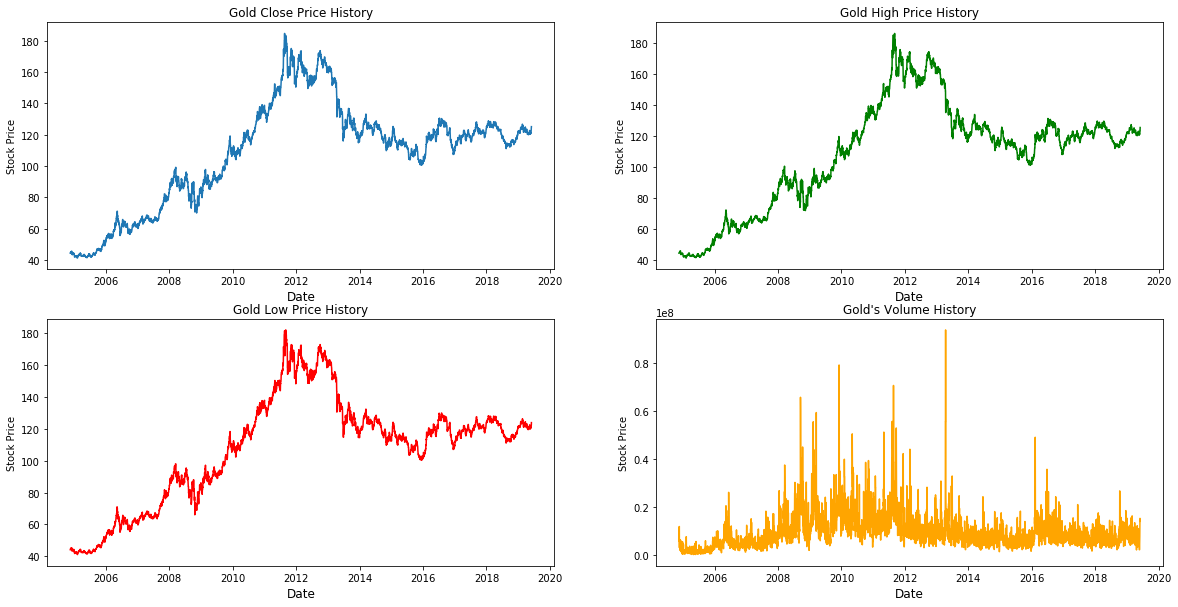
\includegraphics[width=16cm]
    {figure/data/plot.png}}
    \caption{\label{fig:gld-data} Biểu đồ dữ liệu}
\end{figure}

Dữ liệu được lấy từ ngày \textbf{18-11-2004} đến \textbf{06-03-2019}. 
Dữ liệu được lấy từ thị trường chứng khoán, chính vì vậy, có những ngày nghỉ như ngày lễ, ngày thứ 7, chủ nhật sẽ không có dữ liệu.
Có vẻ như dữ liệu không có tính thời vụ trong năm, tính thời vụ trong mùa và không bị ảnh hưởng bởi ngày lễ. Số lượng bán ra không phụ thuộc vào giá.

\subsection{Xử lý dữ liệu}

\textbf{Đối với mạng học sâu} \\
Chuyển thành bài toán học có giám sát
\begin{itemize}
    \item Đối với những ngày không có dữ liệu thì điền dữ liệu bằng ngày trước để có tính liên tục \\
    \item Giữ lại cột: Date, Close. Đổi tên cột Date thành ds, Close thành y. Bỏ các cột còn lại(Theo quy chuẩn) \\
    \item Chuẩn hoá dữ liệu cột y bằng MinMaxScalar với khoảng (0, 1) \\
    \item Giữ 90 ngày cuối để xác minh. Những ngaỳ còn lại để đem train \\
	\item Đối với mỗi ngày, dữ liệu đầu vào: sẽ ra giá của 90 ngày trước ngày hiện tại, dữ liệu đầu ra là giá vàng của ngày hiện tại +  89 ngày sau ngày hiện tại. Vậy sẽ bỏ qua 90 ngày đầu của bộ dữ liệu (thiếu dữ liệu ngày trước đó). 90 ngày cuối vẫn giữ lại. Đối với những ngày không có dữ liệu thì điền vào 0 \\
	\begin{figure}[h]
		\center{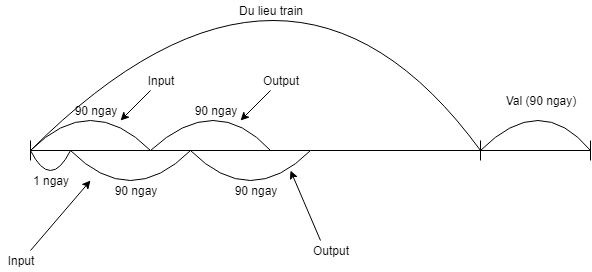
\includegraphics[width=16cm]
		{figure/preprocessing.png}}
		\caption{\label{fig:preprocessing} Mô tả dữ liệu đâù vào đầu ra}
	\end{figure}
\end{itemize}
\begin{table}[h]
	\begin{tabularx}{\textwidth}{X | X | X | X | X | X | X } 
		%\hline
		y\_past\_1	& y\_past\_2	 & y\_past\_3	& ...	& y\_past\_88	 & y\_past\_89	 & y\_past\_90 		\\ \hline
		0.009210	& 0.009000	& 0.005721	& ... & 0.024559	& 0.024559	& 0.021768\\ \hline
		...	& ...	& ...	& ... & ...	& ...	& ... \\ \hline
		0.512300	& 0.540010	& 0.531230	& ... & 0.550120	& 0.550300	& 0.550309\\ %\hline
	\end{tabularx}
	\label{tab:table_input}
	\caption{Dữ liệu đầu vào mẫu}
\end{table}
\begin{table}[h]
	\begin{tabularx}{\textwidth}{X | X | X | X | X | X | X } 
		%\hline
		y	& y\_future\_1 & y\_future\_2	& ...	& y\_future\_87	 & y\_future\_88	 & y\_future\_89		\\ \hline
		0.008791	& 0.010256	& 0.010396		& ... & 0.004814	& 0.004814	& 0.004326\\ \hline
		...	& ...	& ...	& ... & ...	& ...	& ... \\ \hline
		0.520001	& 0	& 0		& ... & 0	& 0	& 0\\ %\hline
\end{tabularx}
	\label{tab:table_output}
	\caption{Dữ liệu đầu ra mẫu}
\end{table}

\clearpage
\textbf{Đối với Prophet}
Chỉ cần đưa dữ liệu vào
\begin{itemize}
    \item Đối với những ngày không có dữ liệu thì điền dữ liệu bằng ngày trước để có tính liên tục \\
    \item Giữ lại cột: Date, Close. Đổi tên cột Date thành ds, Close thành y. Bỏ các cột còn lại(Theo quy chuẩn) \\
    \item Giữ 90 ngày cuối để xác minh. Những ngày còn lại để đem train \\
\end{itemize}
\begin{table}[h]
	\begin{tabularx}{\textwidth}{X | X } 
		%\hline
		ds	& y	  \\ \hline
		2019-03-01	& 121.879997 \\ \hline
		2019-03-02	& 121.879997 \\ \hline
		2019-03-03	& 121.823122 \\ \hline
		2019-03-04	& 121.842212 \\ \hline
		2019-03-05	& 121.851212 \\ %\hline
	\end{tabularx}
	\label{tab:data_prophet}
	\caption{Dữ liệu mẫu Prophet}
\end{table}

\subsection{Xây dựng mô hình}
\textbf{Mạng học sâu} \\
Mạng học sâu 1 là mạng LSTM chồng chất gồm 5 lớp: LSTM -> Dropout -> LSTM -> Dropout -> Dense \\
\begin{minted}{python}
complex_model = Sequential()
complex_model.add(LSTM(units=100, input_shape=(X_train_vals.shape[1],
X_train_vals.shape[2]), return_sequences=True))
complex_model.add(Dropout(rate=0.2))
complex_model.add(LSTM(100, return_sequences=False))
complex_model.add(Dropout(rate=0.2))
complex_model.add(Dense(prediction_size, activation='linear'))
complex_model.compile(loss='mae', optimizer='adam')
\end{minted}
Mạng học sâu 2 lúc sau đơn giản hơn là : LSTM -> Dense \\
\begin{minted}{python}
basic_model = Sequential()
basic_model.add(LSTM(500, input_shape=(X_train_vals.shape[1],
X_train_vals.shape[2])))
basic_model.add(Dense(prediction_size))
basic_model.compile(loss='mae', optimizer='adam')
\end{minted}
Đầu vào có dạng (90, 1) \\
Đầu ra có dạng (90) (dự đoán 90 ngày cùng lúc) \\
Mạng được train với loss function là \(MAE = \frac{1}{n}\sum_{i=1}^{n}|p_i - a_i|\), optimizer là Adam, số epochs là 60 \\
\textbf{Prophet} \\
Prophet với tham số mặc định, sử dụng daily seasonality, weekly seasonality, daily seasonality \\
\begin{minted}{python}
m = Prophet(yearly_seasonality=True, 
weekly_seasonality=True, daily_seasonality=True)
\end{minted}
\subsection{Phương pháp đánh giá}
Trong bài toán dự đoán này, ta sử dụng \textbf{Walk Forward Validation}.
Có một vài cần quyết định quyết định để đưa ra:
\begin{enumerate}
	\item \textbf{Số lượng dữ liệu tối thiểu}: Đầu tiên, chúng ta phải chọn số lượng dữ liệu tối thiểu cần thiết để huấn luyện mô hình. Điều này có thể được coi là chiều rộng cửa sổ nếu sử dụng cửa sổ trượt.
	\item \textbf{Cửa sổ trượt hoặc mở rộng}: Tiếp theo, chúng ta cần quyết định liệu mô hình sẽ được đào tạo trên tất cả dữ liệu mà nó có sẵn hay chỉ trên các dữ liệu gần đây nhất. Điều này xác định xem một cửa sổ trượt hoặc mở rộng sẽ được sử dụng.
\end{enumerate}

Sau khi chọn cấu hình hợp lý, ở bài toán này là cửa sổ mở rộng, các mô hình có thể được đào tạo và đánh giá.
\begin{enumerate}
	\item Bắt đầu từ đầu chuỗi thời gian, số lượng mẫu tối thiểu trong cửa sổ được sử dụng để huấn luyện một mô hình.
	\item Mô hình đưa ra dự đoán cho bước tiếp theo.
	\item Dự đoán được lưu trữ hoặc đánh giá theo giá trị đã biết.
	\item Cửa sổ được mở rộng để bao gồm giá trị đã biết và quy trình được lặp lại (chuyển sang bước 1.)
\end{enumerate}

Có thể hình dung như hình minh hoạ sau đây:
\begin{figure}[h]
    \center{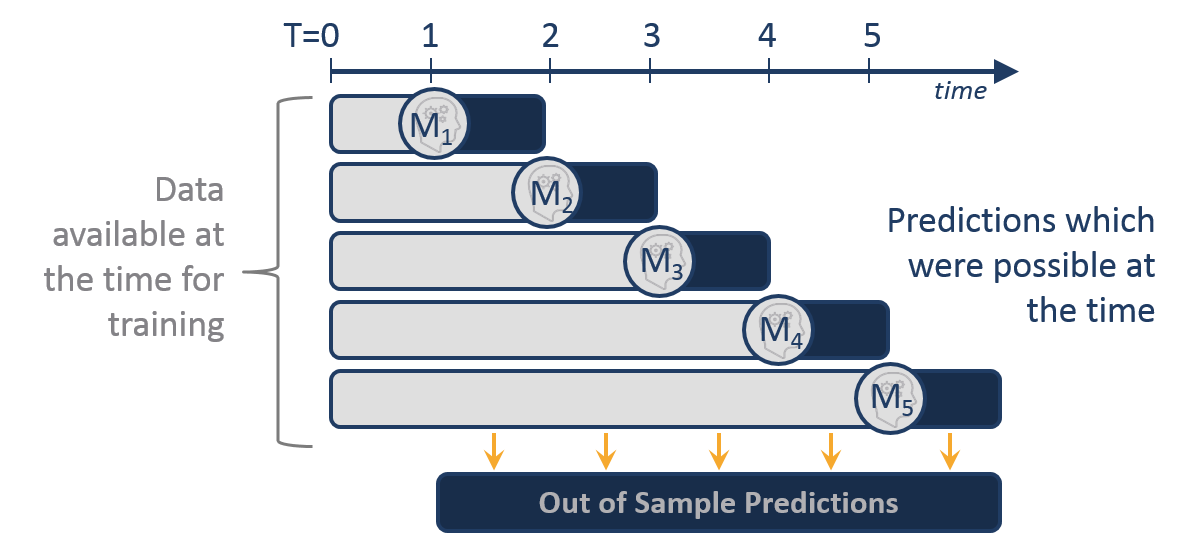
\includegraphics[width=10cm]
    {figure/walkforward.png}}
    \caption{\label{fig:walkforward} Minh hoạ Walk Forward Validation}
\end{figure}

Sử dụng công thức MAE để đánh giá. \\
\[MAE = \frac{1}{n}\sum_{i=1}^{n}|p_i - a_i|\]
\begin{minipage}[t]{.27\textwidth}
	\textit{Trong đó}
\end{minipage}
\hspace*{15pt}
\begin{minipage}[t]{.65\textwidth}
	\(n\) là số ngày dự đoán \\
	\(p_i\) là kết quả dự đoán vào ngày thứ \(i\) \\
	\(a_i\) là kết quả thực tế vào ngày thứ \(i\) \\
\end{minipage} \\[5mm]

Lấy 90 ngày cuối trong bộ dữ liệu để xác minh. Ta được kết quả như bảng sau: \\

\begin{table}[h]
	\begin{tabularx}{\textwidth}{X | X }
		%\hline
		Mô hình	& MAE	  \\ \hline
		Mạng học sâu 1 LSTM chồng chất	& 4.3483 \\ \hline
		Mạng học sâu 2 đơn giản	& 1.1131 \\ \hline
		Prophet	& 1.2269 \\
	\end{tabularx}
	\label{tab:result}
	\caption{Kết quả}
\end{table}
\begin{figure}[h]
    \center{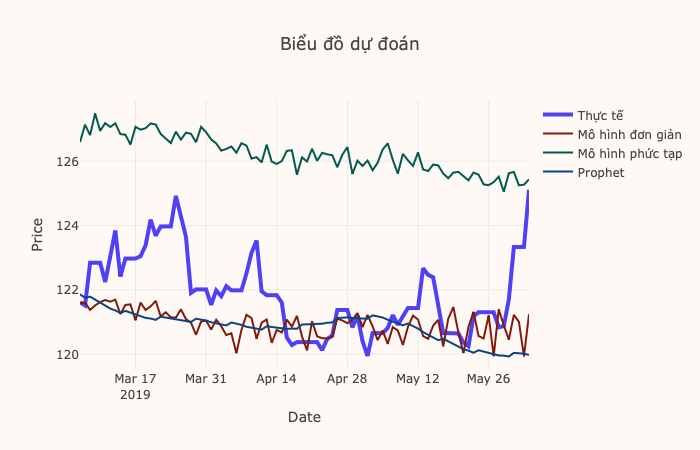
\includegraphics[width=16cm]
    {figure/result.png}}
    \caption{\label{fig:result-chart} Biểu đồ kết quả xác minh 90 ngày cuối}
\end{figure}

Tính trung bình MAE trong các bước \textbf{Walk Forward Validation}, với mỗi bước tăng thêm 360 mẫu dữ liệu để đự đoán 90 ngày sau. Ta được kết quả như bảng sau: \\

\begin{table}[h]
	\begin{tabularx}{\textwidth}{X | X }
		%\hline
		Mô hình	& MAE	  \\ \hline
		Mạng học sâu 1 LSTM chồng chất & 17.1441 \\ \hline
		Mạng học sâu 2 đơn giản & 16.0428 \\ \hline
		Prophet	& 5.9291 \\
	\end{tabularx}
	\label{tab:resulttimewalking}
	\caption{Kết quả \textbf{Walk Forward Validation}}
\end{table}

Prophet không tinh chỉnh nhiều tham số gì lại đưa ra kết quả chính xác hơn mạng LSTM chồng chất.


\section{Recurrent neural network}
\label{sec:intro:lstm}
Con người không bắt đầu suy nghĩ từ đầu mỗi giây.
Khi bạn đọc bài luận này, bạn hiểu từng từ dựa trên sự hiểu biết của bạn về các từ trước đó.
Bạn không nên ném mọi thứ đi và bắt đầu suy nghĩ lại từ đầu. Suy nghĩ của bạn
có sự lưu lại.

Mạng lưới thần kinh truyền thống có thể làm được điều này, và nó có vẻ như là một
thiếu sót lớn.
Ví dụ, hãy tưởng tượng bạn muốn phân loại loại sự kiện nào đang diễn ra tại mọi thời điểm trong phim.
Nó không rõ làm thế nào một mạng lưới thần kinh truyền thống có thể sử dụng lý lẽ của nó về các sự kiện trước đó trong phim để thông báo cho những sự kiện sau này.

Recurrent neural network giải quyết vấn đề này. Chúng là các mạng có các vòng lặp trong đó, cho phép thông tin tồn tại.
\begin{figure}[H]
    \center{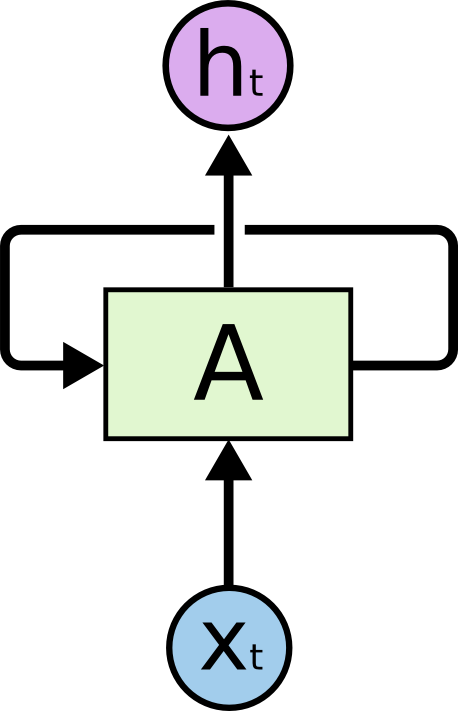
\includegraphics[width=4cm]
    {figure/model/RNN-rolled.png}}
    \caption{\label{fig:rnn-rolled} Recurrent Neural Network có vòng lặp.}
\end{figure}

Trong sơ đồ trên, một đoạn của mạng thần kinh, \(A\), xem xét một số \(x_t\) đầu vào và xuất ra một giá trị
\(h_t\).Một vòng lặp cho phép thông tin được truyền từ một bước của mạng sang bước tiếp theo.

Những vòng lặp này làm cho Recurrent neural network có vẻ như bí ẩn.
Tuy nhiên, nếu bạn suy nghĩ nhiều hơn một chút, hóa ra họ không phải là một mạng lưới thần kinh bình thường.
Recurrent neural network có thể được coi là nhiều bản sao của cùng một mạng, mỗi bản tin truyền cho một người kế nhiệm.
Xem xét những gì xảy ra nếu chúng ta bỏ vòng lặp:

\begin{figure}[H]
    \center{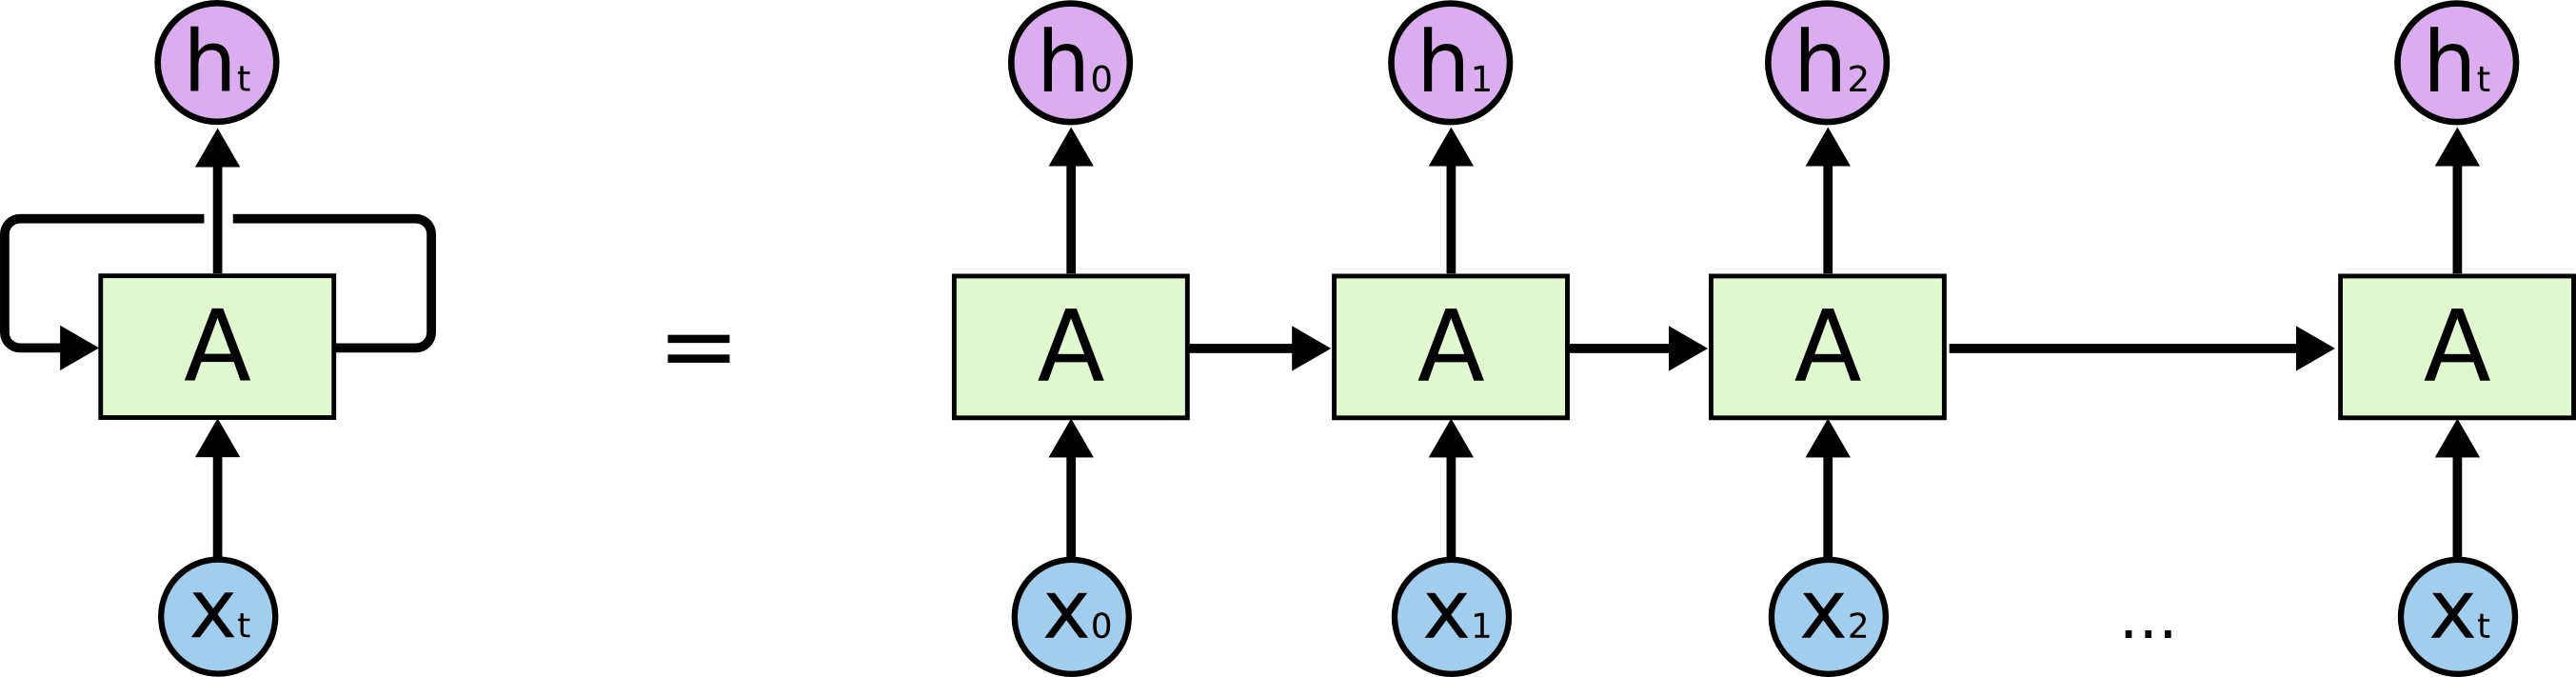
\includegraphics[width=\figureBigSize]
    {figure/model/RNN-unrolled.png}}
    \caption{\label{fig:rnn-unrolled} Recurrent Neural Network đã được trải ra.}
\end{figure}

Bản chất giống như chuỗi này cho thấy các Recurrent neural network có liên quan mật thiết đến các chuỗi và danh sách.
Nó sử dụng kiến trúc tự nhiên của mạng neuron để sử dụng cho dữ liệu đó.

Và chúng chắc chắn được sử dụng!
Trong vài năm qua, đã có những thành công đáng kinh ngạc khi áp dụng RNN cho nhiều vấn đề khác nhau: nhận dạng giọng
nói, mô hình ngôn ngữ, dịch thuật, chú thích hình ảnh.

Điều cần thiết cho những thành công này là việc sử dụng "LSTM", một loại Recurrent neural network rất đặc biệt, hoạt
động, cho nhiều tác vụ, tốt hơn nhiều so với phiên bản tiêu chuẩn. Hầu như tất cả các kết quả thú vị dựa trên Recurrent neural network đều đạt được với chúng. Nó có những LSTM mà bài tiểu luận này sẽ khám phá.

\textbf{Vấn đề phụ thuộc xa} \\[0.2em]
Một trong những lời kêu gọi của RNN là ý tưởng rằng họ có thể kết nối thông tin trước đó với tác vụ hiện tại, chẳng
hạn như sử dụng các khung video trước đó có thể thông báo cho sự hiểu biết về khung hiện tại. Nếu RNN có thể làm điều
này, thì họ cực kỳ hữu ích. Nhưng họ có thể? Không hẳn.

Đôi khi, chúng ta chỉ cần nhìn vào thông tin gần đây để thực hiện nhiệm vụ hiện tại. Ví dụ, hãy xem xét một mô hình
ngôn ngữ đang cố gắng dự đoán từ tiếp theo dựa trên các từ trước đó. Nếu chúng ta đang cố gắng dự đoán từ cuối cùng
trong "các đám mây trên \textit{bầu trời}", thì chúng ta không cần bất kỳ bối cảnh nào nữa - đó là một điều khá rõ ràng,
từ tiếp theo sẽ là  \textit{bầu trời}. Trong những trường hợp như vậy, khi khoảng cách giữa thông tin liên quan và
địa điểm mà nó cần là nhỏ, RNN có thể học cách sử dụng thông tin trong quá khứ.

\begin{figure}[H]
    \center{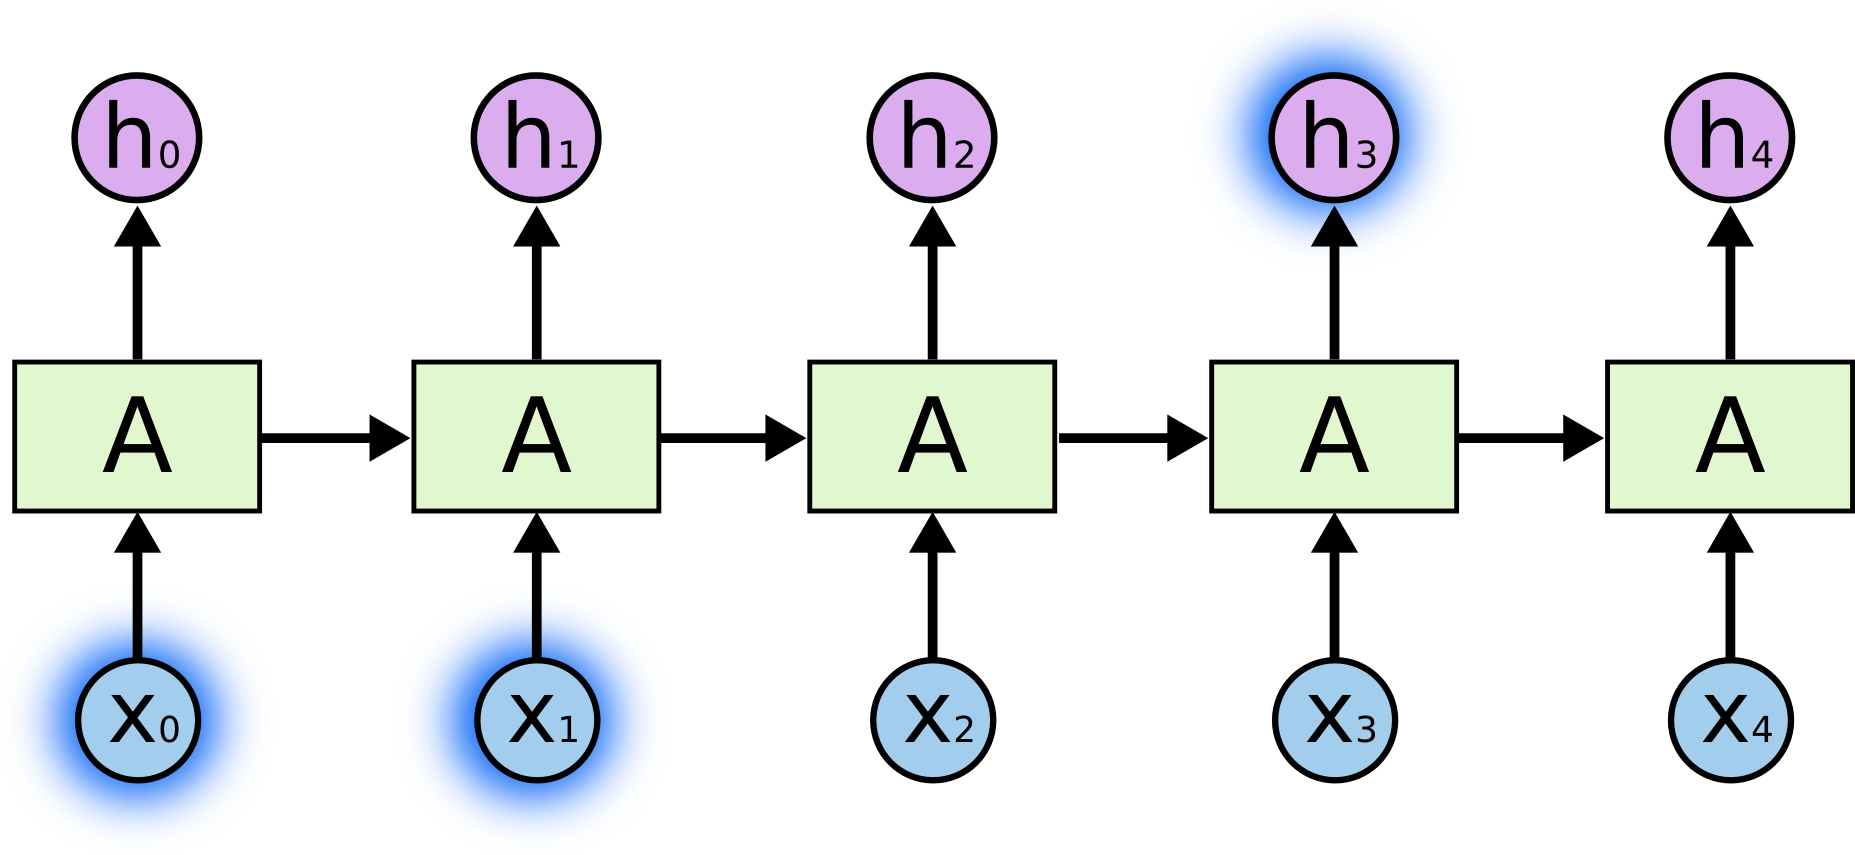
\includegraphics[width=\figureBigSize]
    {figure/model/RNN-shorttermdepdencies.png}}
\end{figure}

Nhưng cũng có những trường hợp chúng ta cần nhiều bối cảnh hơn. Cân nhắc việc cố gắng dự đoán từ cuối cùng trong văn
bản. "Tôi lớn lên ở Việt Nam. Tôi nói tiếng trôi chảy tiếng \textit{Việt}". Thông tin gần đây cho thấy từ tiếp theo có
lẽ là tên của một ngôn ngữ, nhưng nếu chúng ta muốn thu hẹp ngôn ngữ nào, chúng ta cần thu hẹp ngôn ngữ nào bối cảnh
của Việt Nam, từ phía trước. Nó hoàn toàn có thể cho khoảng cách giữa thông tin liên quan và điểm cần thiết để trở
nên rất lớn.

Thật không may, khi khoảng cách đó tăng lên, các RNN trở nên không thể học cách kết nối thông tin.
\begin{figure}[H]
    \center{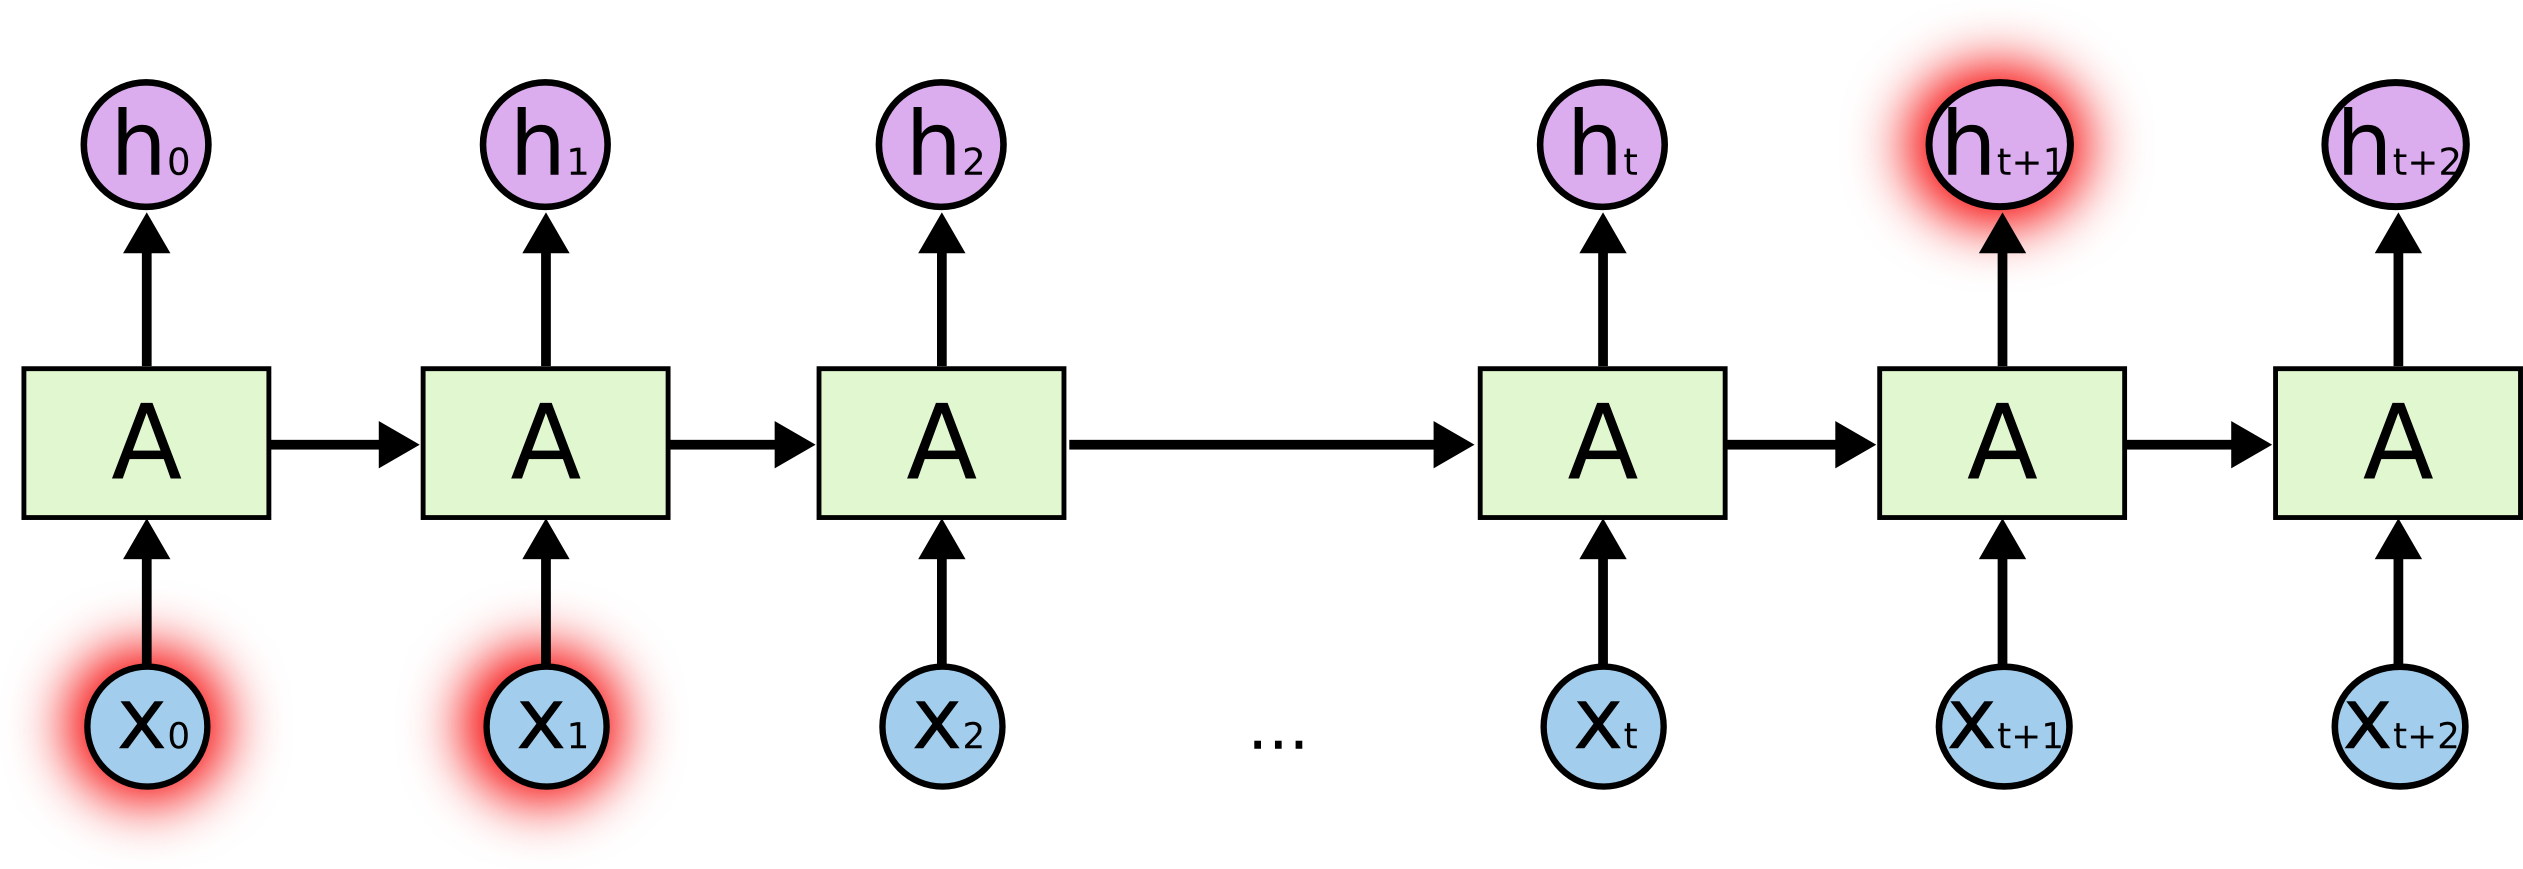
\includegraphics[width=\figureBigSize]
    {figure/model/RNN-longtermdependencies.png}}
\end{figure}


Về lý thuyết, các RNN hoàn toàn có khả năng xử lý các phụ thuộc dài hạn như vậy. Một người có thể cẩn thận chọn các
tham số cho họ để giải quyết các vấn đề theo hình thức này. Đáng buồn thay, trong thực tế, RNN trông
dường như không có thể học chúng. Vấn đề đã được khám phá sâu bởi Hochreiter (1991) [German] và Bengio, et al. (1994),
người đã tìm thấy một số lý do khá cơ bản tại sao nó có thể khó khăn.

Rất may, LSTM không có vấn đề này!

\textbf{Mạng LSTM} \\[0.2em]
Long Short Term Memory (mạng bộ nhớ dài ngắn hạn) - thường được gọi là LSTM của - - là một loại RNN đặc biệt, có khả năng học các phụ thuộc xa. Chúng được giới thiệu bởi Hochreiter \& Schmidhuber (1997), và được nhiều người tinh chỉnh và phổ biến. Chúng hoạt động rất tốt trong nhiều vấn đề lớn, và hiện đang được sử dụng rộng rãi.

Các LSTM được thiết kế rõ ràng để tránh vấn đề phụ thuộc dài hạn. Ghi nhớ thông tin trong thời gian dài thực tế là hành vi mặc định của nó, không phải là thứ khó khăn để học!

Tất cả các mạng thần kinh tái phát có dạng một chuỗi các module lặp lại của mạng thần kinh. Trong các RNN tiêu chuẩn, module lặp lại này sẽ có cấu trúc rất đơn giản, chẳng hạn như một lớp \(tanh\) duy nhất.

\begin{figure}[H]
    \center{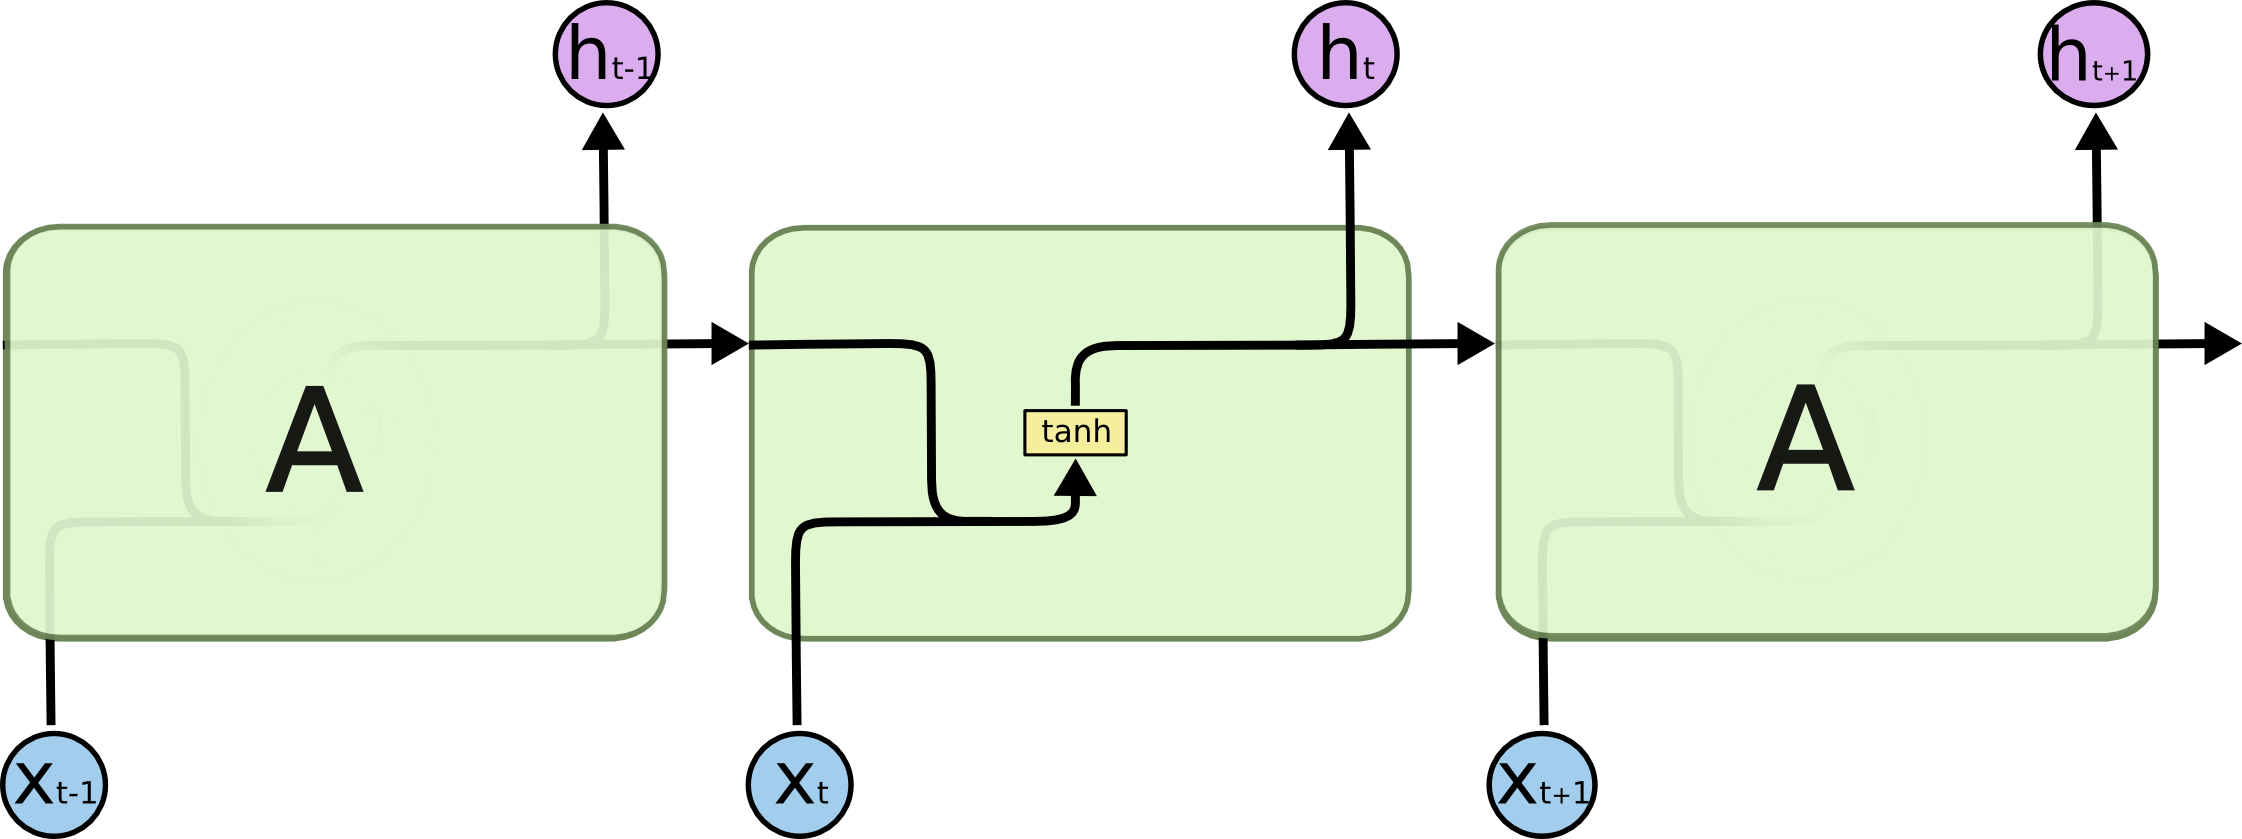
\includegraphics[width=\figureBigSize]
    {figure/model/LSTM3-SimpleRNN.png}}
    \caption{\label{fig:lstm3-simpleRNN} Module lặp trong RNN chuẩn chứa một lớp duy nhất.}
\end{figure}

LSTM cũng có cấu trúc chuỗi, nhưng các module lặp có một cấu trúc khác. Thay vì có một lớp
mạng thần kinh duy nhất,nó có bốn lớp, tương tác theo một cách rất đặc biệt.

\begin{figure}[H]
    \center{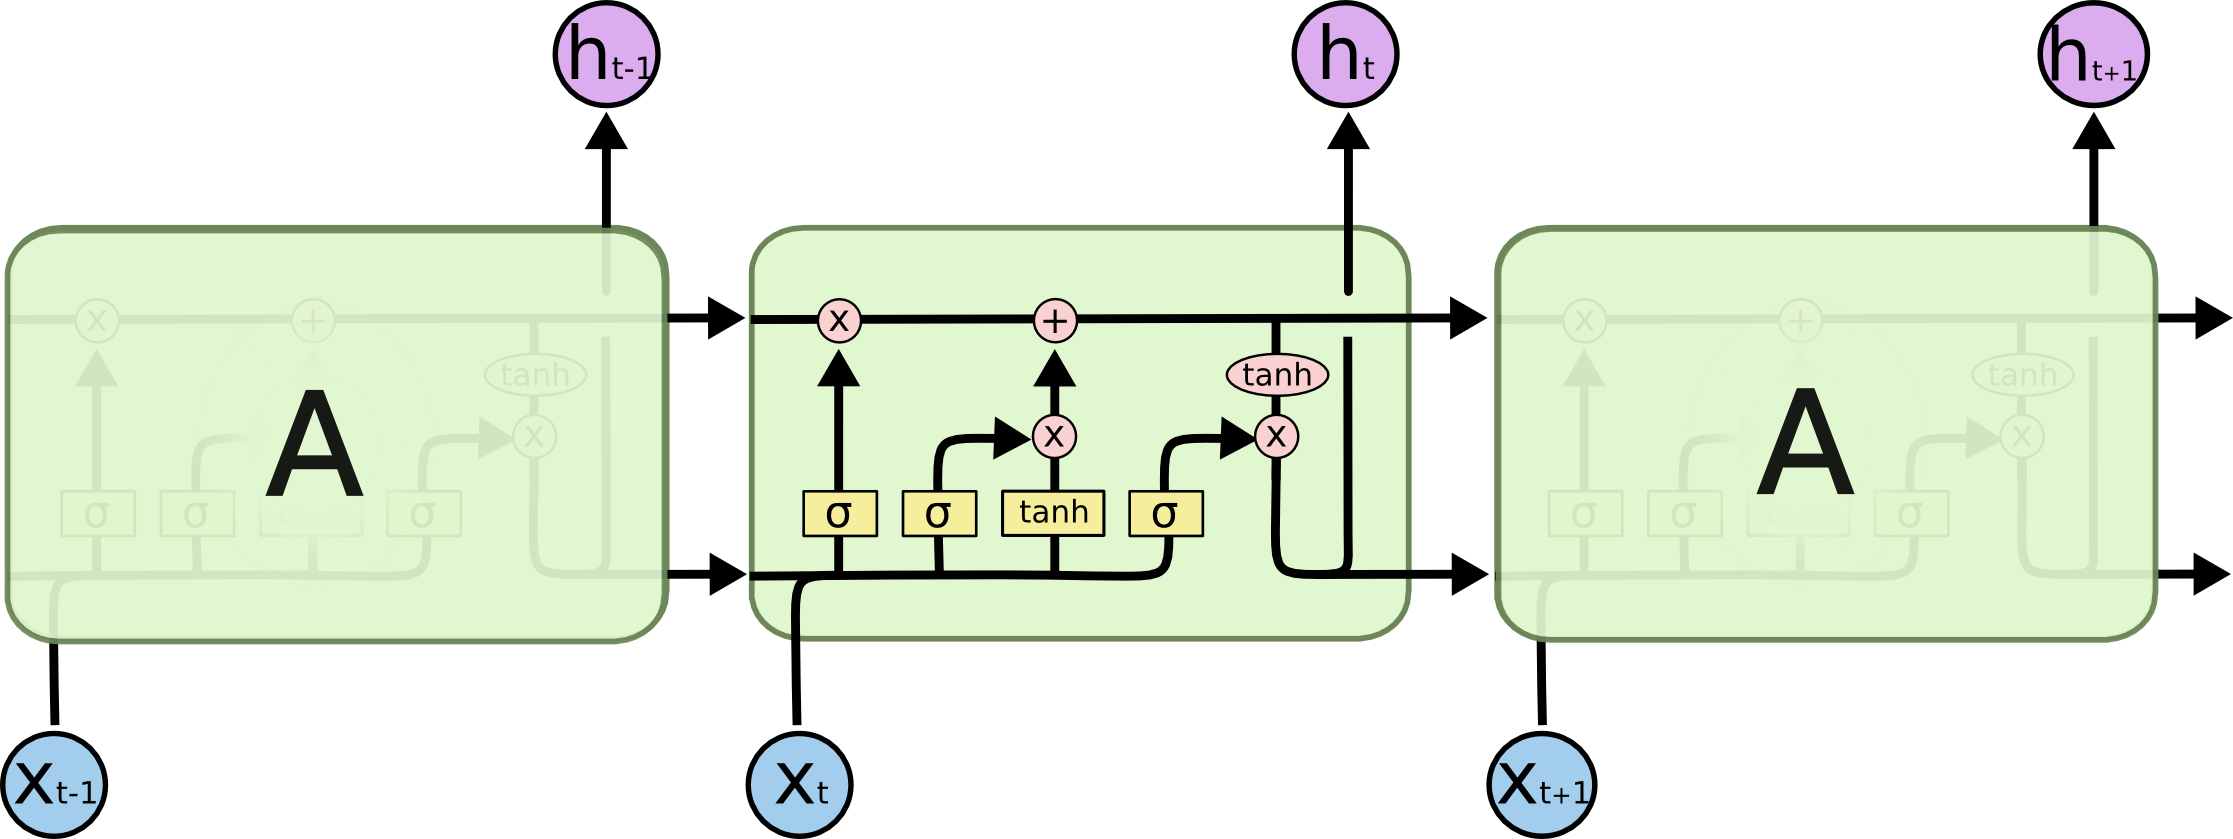
\includegraphics[width=\figureBigSize]
    {figure/model/LSTM3-chain.png}}
    \caption{\label{fig:lstm3-chain} Module lặp trong LSTM chứa 4 lớp tương tác.}
\end{figure}

\begin{figure}[H]
    \center{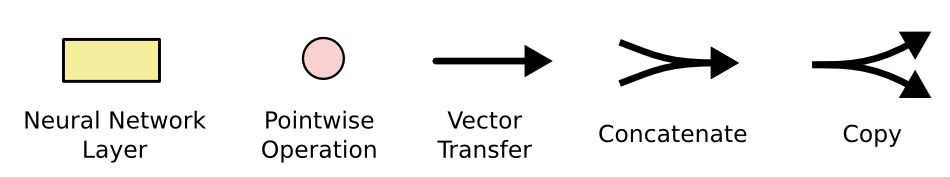
\includegraphics[width=\figureBigSize]
    {figure/model/LSTM2-notation.png}}
    \caption{\label{fig:lstm2-notation} Các ký hiệu trong LSTM.}
\end{figure}

Trong sơ đồ trên, mỗi dòng mang toàn bộ một vector, từ đầu ra của một nút đến đầu vào của các nút khác. Các vòng tròn
màu hồng đại diện cho các phép toán, như phép cộng vector, trong khi các hình chữ nhật màu vàng biểu thị các mạng
thần kinh để học. Các dòng hợp nhất biểu thị việc ghép nối, trong khi một dòng phân tách biểu thị nội dung của nó được
sao chép và các bản sao đi đến các vị trí khác nhau.

\textbf{Ý tưởng chính của LSTM} \\[0.2em]
Ý tưởng chính của LSTM là ô trạng thái, đường ngang chạy qua đỉnh sơ đồ.

Dòng trạng thái giống như một băng chuyền. Nó chạy thẳng xuống toàn bộ chuỗi, chỉ với một số tương tác tuyến tính nhỏ
dọc bên cạnh, dễ dàng cho thông tin truyền theo.

\begin{figure}[H]
    \center{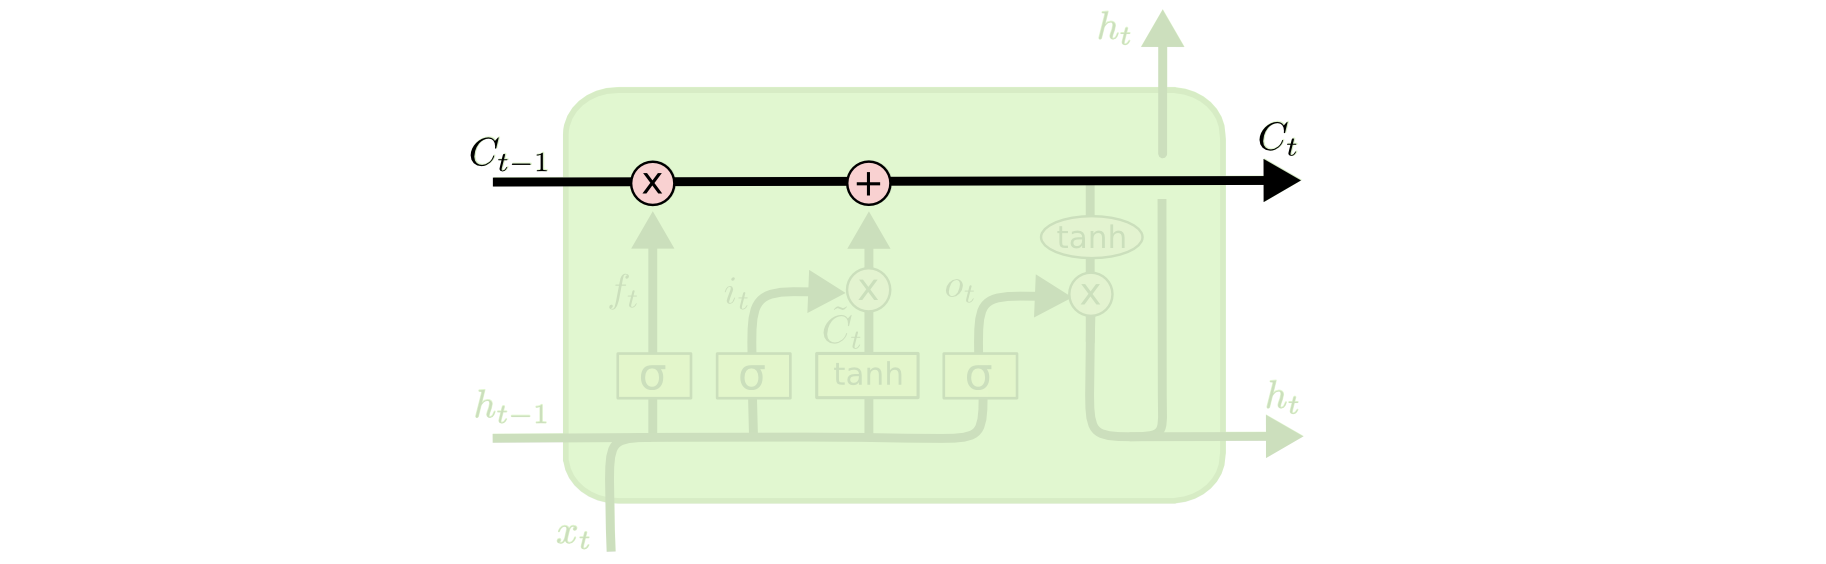
\includegraphics[width=\figureBigSize]
    {figure/model/LSTM3-C-line.png}}
\end{figure}

LSTM có khả năng loại bỏ hoặc thêm thông tin vào ô trạng thái, được điều chỉnh cẩn thận bởi các cấu trúc gọi là
cổng.

Cổng là một cấu trúc điều khiển thông tin thông qua. Chúng được cấu tạo từ một lớp lưới thần kinh \(sigmold\) và
một phép toán nhân.

\begin{figure}[H]
    \center{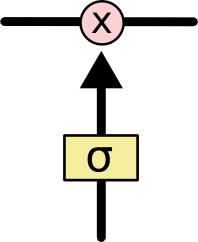
\includegraphics[width=1cm]
    {figure/model/LSTM3-gate.png}}
\end{figure}

Đầu ra của các lớp \(sigmoid\) có giá trị \([0, 1]\), mô tả mức độ cho qua. Giá
trị bằng \(0\) có nghĩa là không để bất cứ thứ gì qua, trong khi giá trị của \(1\) nghĩa
là có thể cho phép mọi thứ thông qua!

Một LSTM có ba trong cổng này, để bảo vệ và kiểm soát trạng thái tế bào.

\textbf{Các bước LSTM hoạt động} \\[0.2em]
Bước đầu tiên trong LSTM  là quyết định thông tin nào đi ra khỏi ô trạng thái. Quyết định này được đưa ra bởi
một lớp sigmoid được gọi là lớp "cổng quên". Nó dựa vào giá trị của \(h_{t-1}\) và \(x_t\), và đưa ra một số từ 0
đến 1 tương ứng với mỗi số ô trạng thái \(c_{t-1}\). Số 1 có nghĩa là giữ lại toàn bộ thông tin trong khi đó số 0 nghĩa
là hãy quên nó đi.

Hãy xem ví dụ của chúng ta về một mô hình ngôn ngữ đang cố gắng dự đoán từ tiếp theo dựa trên tất cả các từ trước đó.
Trong một vấn đề như vậy, ô trạng thái có thể bao gồm vai vế của ngữ hiện tại, để có thể sử dụng các động từ
một cách chính xác. Khi có một chủ ngữ mới, nó sẽ quên đi vai vế của chủ ngữ cũ.

\begin{figure}[H]
    \center{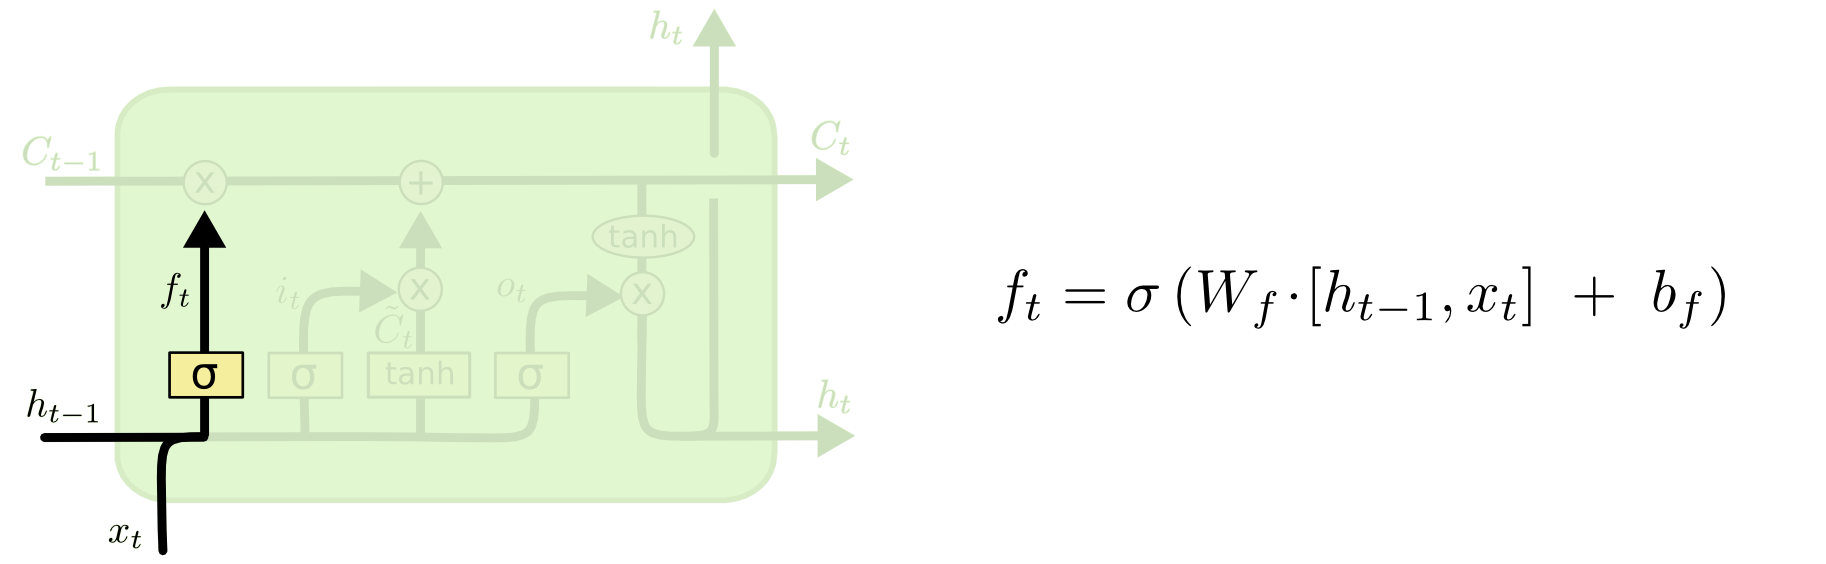
\includegraphics[width=\figureBigSize]
    {figure/model/LSTM3-focus-f.png}}
\end{figure}

Bước tiếp theo là quyết định những thông tin mới sẽ lưu trữ trong ô trạng thái. Việc này có hai phần. Đầu tiên,
một lớp sigmoid được gọi là lớp "cổng đầu vào" quyết định giá trị nào sẽ cập nhật. Tiếp theo, một lớp \(tanh\)
tạo ra một vector các giá trị ứng cử viên mới, \(C_t\), có thể được thêm vào ô trạng thái. Sau đó sẽ kết hợp  cả hai
để tạo ra một bản cập nhật cho trạng thái.

Trong ví dụ về mô hình ngôn ngữ, chúng tôi muốn thêm vai vế của chủ ngữ mới vào ô trạng thái, để thay thế chủ ngữ đã
quên.
\begin{figure}[H]
    \center{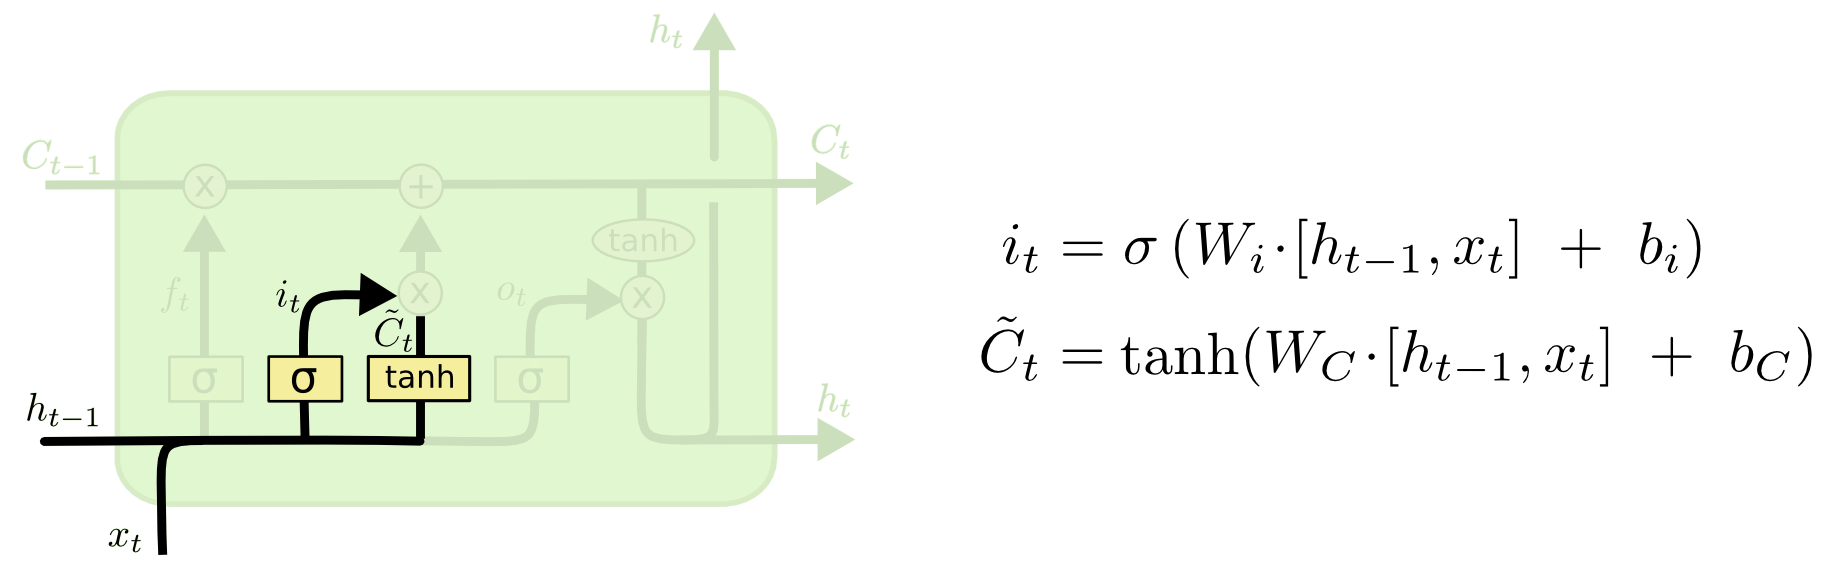
\includegraphics[width=\figureBigSize]
    {figure/model/LSTM3-focus-i.png}}
\end{figure}

Bây giờ, sẽ cập nhật ô trạng thái cũ, \(C_{t-1}\), sang ô trạng thái mới \(C_{t}\). Các bước trước đã quyết định phải
quên và nhớ những gì, giờ là lúc thực hiện nó.

Nhân ô trạng thái cũ với \(f_t\), quên đi những điều quyết định quên trước đó. Sau đó, cộng với \(i_t*\widetilde{C}_t\).
Đây là giá trị ứng viên mới, được tính theo mức độ cập nhật từng giá trị trạng thái.

Trong trường hợp của mô hình ngôn ngữ, đây là lúc thực sự bỏ thông tin về vai vế và thêm thông tin mới, như đã quyết
định trong các bước trước.
\begin{figure}[H]
    \center{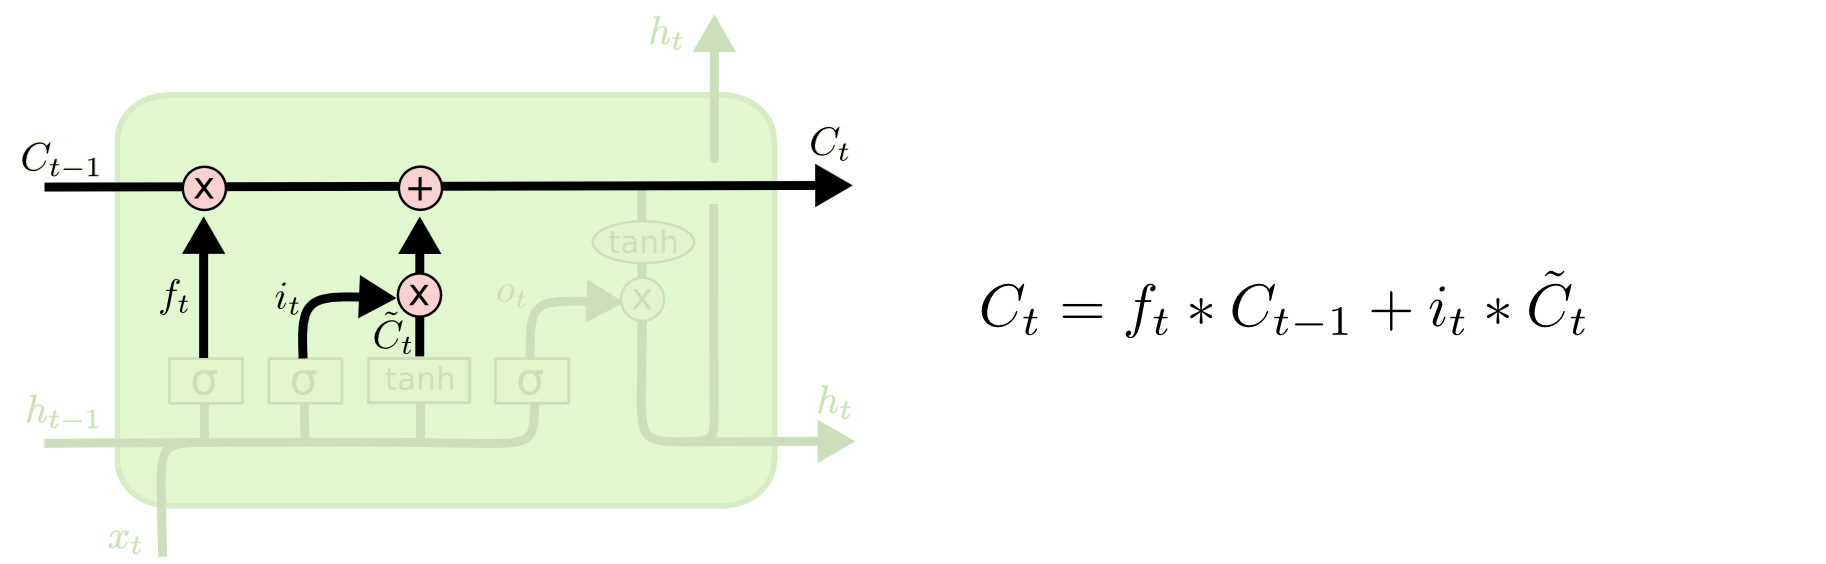
\includegraphics[width=\figureBigSize]
    {figure/model/LSTM3-focus-C.png}}
\end{figure}
Cuối cùng là quyết định những gì sẽ xuất ra. Đầu ra sẽ được lọc dựa vào ô trạng thái. Đầu tiên, chạy một lớp
\(sigmoid\) quyết định phần nào của ô trạng thái mà sẽ xuất ra. Sau đó, đưa ô trạng thái qua hàm
\(tanh\) (để đẩy các giá trị nằm trong khoảng -1 đến 1) và nhân nó với đầu ra của cổng \(sigmoid\), do đó chỉ đưa ra
các dữ liệu đã quyết định

Đối với ví dụ về mô hình ngôn ngữ, vì nó chỉ nhìn thấy một chủ ngữ, nó có thể muốn đưa ra thông tin có liên quan đến
một động từ, trong trường hợp đó là những gì sắp diễn ra. Ví dụ, nó có thể xuất ra vai vế của chủ ngữ , để biết được
cách dùng từ với chủ ngữ đó.
%\input{demo-Chapter2.tex}
%\input{Chapter3.tex}

%-	Danh mục TL tham khảo
%-	Phụ lục (nếu có)

\bibliographystyle{plain} % ieeetr
\bibliography{refs} 

\end{document}
